\documentclass{article}
\usepackage[margin=3cm]{geometry}
\usepackage{amssymb}

% Figures
\usepackage{graphicx}
\usepackage{color}

% Page formatting
\newsavebox{\notetitle}
\newsavebox{\noteauthor}
\newsavebox{\notenumber}
\newsavebox{\notedate}
\renewcommand{\title}[1]{\sbox{\notetitle}{\Large{\textbf{#1}}}}
\renewcommand{\author}[1]{\renewcommand{\and}{\quad}\sbox{\noteauthor}{\large{#1}}}
\renewcommand{\date}[1]{\sbox{\notedate}{\large{#1}}}
\newcommand{\nb}[1]{\sbox{\notenumber}{\Large{\textbf{#1}}}}
\newcommand{\makemadtitle}{
  \hrule
  \vspace{.5em}
  \noindent
  \begin{center}
  \textbf{
  {\centering
\includegraphics[height=3cm]{../logoCHISTERA2014}}\\
   {\centering\Large COACHES project, CHIST-ERA 2014 program}
  }
  \end{center}
  \vspace{.5em}
 
  \hrule
  \vspace{3em}
  \begin{center}
    \begin{large}\textbf{ Note~\usebox{\notenumber}.}\end{large}\\[.5em]
    \begin{Large}\textbf{\usebox{\notetitle}}\end{Large}\\[2em]
    \begin{large}\usebox{\noteauthor} --- \usebox{\notedate}\end{large}
  \end{center}
  \vspace{3em}
}

% Various macros and environments
\newtheorem{prop}{Proposition}
\newtheorem{proposition}[prop]{Proposition}
\newtheorem{defn}{Definition}
\newtheorem{definition}[defn]{Definition}
\newtheorem{cor}{Corollary}
\newtheorem{corollary}[cor]{Corollary}
\newtheorem{exmp}{Example}
\newtheorem{example}[exmp]{Example}
\newtheorem{lem}{Lemma}
\newtheorem{lemma}[lem]{Lemma}
\newtheorem{fact}{Fact}
\newtheorem{thm}{Theorem}
\newtheorem{theorem}[thm]{Theorem}
\newtheorem{prob}{Problem}
\newtheorem{problem}[prob]{Problem}
\newtheorem{rem}{Remark}
\newtheorem{remark}[rem]{Remark}
\newtheorem{conj}{Conjecture}
\newtheorem{conjecture}[conj]{Conjecture}
\newenvironment{pf}{{\bf Proof }}{\hfill$\Box$\par}
\newenvironment{proof}{{\bf Proof }}{\hfill$\Box$\par}
\newcommand{\spaceafterproof}{\vspace{1em}}

% NOTE ITSELF BELOW %%%%%%%%%%%%%%%%%%%%%%%%%%%%%%%%%%%%%%%%%%%%%

\title{D1.1 Knowledge-based environment modelling}
\author{COACHES Consortium: Abdel-Illah, Luca, Esra}
\nb{: Draft D1.1 }

\date{\today}

\begin{document}

\includegraphics[height=2cm]{../fig/logoUNICAEN.jpg}

\includegraphics[height=2cm]{../fig/logoSapienza.png}
%
\includegraphics[height=2cm]{../fig/logoVUB}

\includegraphics[height=2cm]{../fig/logoSebanci}


\makemadtitle

\vspace*{1.0in}
\begin{abstract}
This document describes the general principles of the Knowledge-based representation and reasoning techniques developed in WP1. In particular, it describes the formalism for representing the semantic map of the environment, spatial information, common sense, and events as well as the algorithms for reasoning about this knowledge. 
\end{abstract}

\vspace*{1.5in}

\fbox{
\begin{minipage}{1.0\textwidth}
\begin{center}
 $\copyright$, THE COACHES CONSORTIUM \\
The copyright in this document is the property of the COACHES Consortium. This document is supplied by the COACHES consortium on the express terms that it is to be treated as confidential. This document is not external distribution without the project manager's permission. 
\end{center}
\end{minipage}
}
\newpage
\section{Introduction}
This document consists of describing different principles of the Knowledge-based reasoning module developed in WP1. This  module receives different information from different units, sensors or other modules of the architecture, particularly the multi-modal interface and the perception modules. These information concern the semantic map, spatial information and human activities. From these information, the reasoning module should infer new goals to accomplish. This list of goals is sent the decision module that will compute the behavior policy of the robot to accomplish such goals. The behavior policy is then sent to the executor module based on Petri Net Plans. The general principle is depicted in Figure \ref{WP1principle}.

\begin{figure}[htbp]
\begin{center}
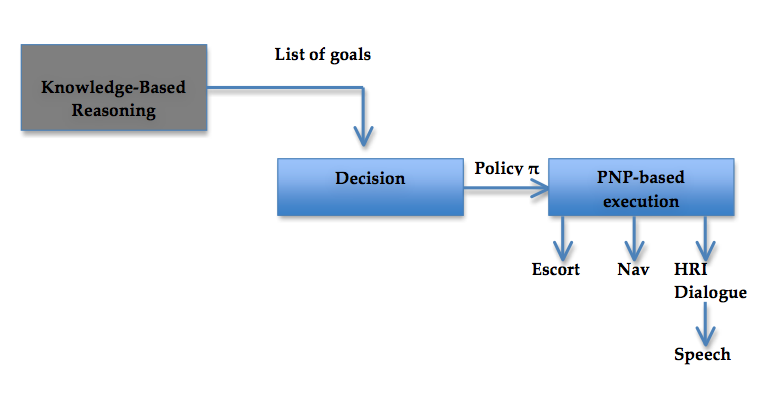
\includegraphics[height=8cm]{WP1Principles}
\caption{General principles of interaction between KB  and decision modules}
\label{WP1principle}
\end{center}
\end{figure}


\section{Design of the knowledge base}

In this section, we define the main features of the knowledge base used in the project. We first introduce the semantic labels used to describe elements of the world, and then predicates that determine relations among these labels.

\subsection{Semantic labels}

In order to refer to objects and classes of objects in the knowledge base, we introduce a set of labels that will be associated to semantic meanings. 

A first set of these labels are called \emph{Concepts} and they are associated to classes of objects. For example, \emph{Restaurant} is a concept used in the semantic map to denote the class of restaurants in the shopping mall. Concept labels always start with an uppercase letter.
These concepts are organized in a hierarchical way according to the ``is-a'' relation.
In this way, we can express, for example, that the concept \emph{FrenchRestaurant} is a \emph{Restaurant}. 

A second set of labels will be used to denote objects. Each object belongs to a concept implementing the relation ``instance-of''. Object labels always start with a lowercase letter.
Thus, a particular restaurant in the mall will be denoted with an object label \emph{caf\'eMarcel} that will be instance of the concept \emph{FrenchRestaurant}. 


\subsection{Predicates}

Predicates are used to describe relations among the semantic labels. For example, the ``is-a'' and the ``instance-of'' relations can be represented by the corresponding predicates {\tt\bf is-a} and {\tt\bf instance-of}. For example, we can write

\begin{quote}
{\tt\bf is-a} ( FrenchRestaurant, Restaurant )\\
{\tt\bf instance-of} ( caf\'eMarcel, FrenchRestaurant )\\
\end{quote}

Sometimes,  the ``is-a'' and the ``instance-of'' relations will be abbreviated respectively by
the operators $\subset$ and $\in$.
Thus, the above example can also be described as \emph{FrenchRestaurant} $\subset$ \emph{Restaurant} and \emph{caf\'eMarcel} $\in$ \emph{FrenchRestaurant}.


Predicates are also used to denote properties of objects. For example, given the concepts \emph{Color} and \emph{Dress} and the objects \emph{red} $\in$ \emph{Color} and \emph{dress\_123} $\in$ \emph{Dress}, the predicate 

\begin{quote}
{\tt\bf color} ( dress\_123,  red )
\end{quote}

\noindent
will represent the color property \emph{red} of the particular object  \emph{dress\_123}.


\section {Representation of the environment}

In this section we present the main concepts (as defined in the previous section) we will consider to represent the status of the environment and to detect events due to external units or human activities. To this end, we consider three types of information: the semantic map, spatial information and human activities.

\subsection {Semantic map}

For the mall map, we consider different types of areas: shops, restaurants, halls, corridors, rest areas, offices, toilettes, etc. For shops, services and restaurants we consider different categories:
\begin{itemize}
\item {\it Shop categories}: dress shop , women dress shop, kid dress shop, men dress shop, makeup store, store perfume, sport store, etc.
\item {\it Restaurant categories}: French, Japanese, Chinese, Italian, Oriental, African, fast-food, etc.
\item {\it Service categories}: security, information, health-care, etc.
\end{itemize}

All these areas are represented as concepts that are grouped in a more general concept \emph{Area}. The hierarchy of these areas will be defined through the ``is-a'' relation of the semantic labels described before.

Doors are also considered as connections of these areas. \emph{Door} is a concept containing door objects and connections of areas through doors are represented with the {\tt\bf connect} predicate.

\begin{quote}
{\bf\tt connect} ( door12, area1, area2 )
\end{quote}

\noindent
where \emph{door12} $\in$ \emph{Door} \emph{area1}, \emph{area2} $\in$ \emph{Area}  are objects belonging to the corresponding concepts. Moreover, the status of the door can be expressed with a predicate {\tt\bf open}. For example,

\begin{quote}
{\tt\bf open}(door12) \\
\end{quote}




% LI replaced by is-a and instance-of
%\subsection{Type predicate}
%{\tt\bf type}(id, door $\|$ shop $\|$ restaurant $\|$ service $\|$ caf� $\|$ corridor $\|$ rest $\|$ wc)
%\subsection{Category predicate}
%{\tt\bf category}(shop\_id, kid\_dress $\|$ men\_dress$\|$woman\_dress $\|$ dress $\|$ sport $\|$ perfume $\|$ decoration)\\
%{\tt\bf category}(restaurant\_id, fastfood $\|$Italian$\|$French $\|$Chinese $\|$Japenese $\|$ Orient)\\
%{\tt\bf category}(service\_id, Security$\|$information $\|$ healtcare)\\



\paragraph*{\bf Example}~\\

\begin{quote}
{\tt\bf is-a}(FrenchRestaurant, Restaurant) \\
{\tt\bf instance-of}(caf\'eMarcel, FrenchRestaurant) \\
{\tt\bf instance-of}(main\_entrance\_ouest\_1, Door) \\
{\tt\bf instance-of}(hall\_rive\_marin, Hall) \\
\end{quote}


For all the areas, we have to define their localization using a global position referred to a metric map of the environment. We assume to have a 2D absolute reference system in the environment, that will be provided by a 2D SLAM module. Position coordinates of areas and objects are thus expressed in this absolute reference system.

The {\tt\bf position} predicate is used to denote the position of an area or an object in the environment.

\begin{quote}
{\tt\bf position}(area, coordinates)
\end{quote}

\noindent
where \emph{area} $\in$ \emph{Area} and \emph{coordinates} is in general a 2D bounding box of the area, that will enclose the region associated to this area. More precisely, \emph{coordinates} is a sequence of $n$ 2D points in absolute coordinates representing a closed polygon: \emph{coordinates} $\equiv \langle (x_1, y_1) , \ldots, (x_n, y_n) \rangle$.

The {\tt\bf position} predicate is also used to represent a unique position of an object for which the size is not important or it is known or estimated (e.g., a person or a robot). In this case \emph{coordinates} is expressed with only one 2D point. 




\subsection{Spatial relations}

In this section we consider all spatial relations and information:
\begin{itemize}
\item {\tt\bf Infrontof}(person\_id, area\_id)
\item {\tt\bf Nearby}(person\_id, area\_id)
\item {\tt\bf At}(person\_id, location)
\item {\tt\bf In}(person\_id $\|$ object\_id, areas\_id)
 \end{itemize}
\subsection{Human activities}
\begin{itemize}
\item {\tt\bf Motionless}(person\_id, time\_t, location)
\item {\tt\bf Request} (request\_id,request\_type, person\_id, location\_t) where {\it Request\_type}  could be escorting\_to(location),informing\_about(area\_id), guiding\_to(location)
\item {\tt\bf Rest\_Area} (person\_id, time\_t, location)
 \end{itemize}
  \subsection{Commonsense and event-based Reasoning}
  \subsubsection{Event Definition}
  \begin{defn}
  An {\bf Event} is a tuple defined by the actor of the event, where the event has been occurred, when and what is the semantic of the event described by spatio-temporal relations or human activities. 
  \[ Event = <actor, location, time, semantic> \] 
  where semantic = At $\|$ In $\|$ Infrontof $\|$ motionless $\|$ rest\_area $\|$ request \\
  \end{defn}
   \subsubsection{Event-based reasoning and goal generation}
   From the list of predicates and events, we create a list of goals to send to the decision module. In the following these are some commonsense rules to generate goals. 
   \begin{itemize}
\item  {\bf joint escorting goal generation}: \\
  If request\_type=escorting\_to(location) and in(location,hall\_id1) and in(robot, hall\_id2) and hall\_id1 $\neq$ hall\_id2 then \\
  add(list\_goal, create\_task (task\_id joint\_escorting\_task, hall\_id2, hall\_id1, location))
\item  {\bf Surveillance goal generation} \\
  If event(object\_id,location,time\_t,in(object\_id,hall\_id)) then \\
  add(list\_goal, create\_task(task\_id, surveillance\_task, location, object\_id))
\item {\bf Advertising goal generation} \\
   If event(person\_id,location,time\_t,infrontof(person\_id, shop\_id) then \\
   add(list\_goal, create\_task(task\_id, advertising\_task, location, person\_id, shop\_id)
\item $\dots$
   \end{itemize}
   
  \section{Conclusion}
  
  This draft describes in an abstract way what we can expect to have in the KB module. Many concepts should be defined and deepened to provide an effective reasoning module. Representation and reasoning techniques should be discussed. Many commonsense reasoning rules should be defined, spatial reasoning and computation of spatial relations from robot and people locations have to be defined. This could also be discussed in the next phone meeting.
     
\end{document}
